\documentclass[10pt]{article}
\usepackage{geometry}
\geometry{a4paper}
\pagestyle{myheadings}
\usepackage{tikz}
\usepackage{pgfplots}
\usepackage{array}  % for table column M
\usepackage{makecell} % to break line within a cell
\usepackage{verbatim}
\usepackage{graphicx}
\usepackage{epstopdf}
\usepackage{amsmath}
\usepackage{amsfonts}
\usepackage{xcolor}
\usepackage{ifthen}
\usepackage{setspace}
\usepackage{placeins} % for FloatBarrier
\usepackage[makeroom]{cancel}
\usepackage[absolute,overlay]{textpos}
\usetikzlibrary{calc, angles,quotes}
\usetikzlibrary{pgfplots.fillbetween, backgrounds}
\usetikzlibrary{positioning}
\usetikzlibrary{arrows}
\usetikzlibrary{pgfplots.groupplots}
\usetikzlibrary{arrows.meta}
\usetikzlibrary{plotmarks}
\usetikzlibrary{decorations.markings}

\usepgfplotslibrary{groupplots}
\pgfplotsset{compat=newest} 

\DeclareGraphicsExtensions{.pdf,.png,.jpg}
\graphicspath{{../figs/}}

\definecolor{blue2}{RGB}{51, 105, 232}  
\definecolor{red2}{RGB}{213, 15, 37}  
\definecolor{green2}{RGB}{0, 153, 37}  

\definecolor{matlabcomment}{RGB}{34,139,34}

\pgfmathdeclarefunction{gauss}{1}{%
	\pgfmathparse{1/(sqrt(2*pi))*exp(-((#1)^2)/2)}%
}

\pgfmathdeclarefunction{laplacian}{2}{%
	\pgfmathparse{1/(#2*2)*exp(-(abs(x-#1))/(#2))}%
}

\pgfmathdeclarefunction{pretty_func}{1}{%
	\pgfmathparse{cos(deg(#1/2)) - sin(deg(#1)) + cos(deg(#1/2)-45) - sin(deg(#1/4)-154)}%
}

\pgfplotsset{
	dirac/.style={
		mark=triangle*,
		mark options={scale=2},
		ycomb,
		scatter,
		visualization depends on={y/abs(y)-1 \as \sign},
		scatter/@pre marker code/.code={\scope[rotate=90*\sign,yshift=-2pt]}
	}
}

\def\thickness{very thick}

\tikzset{
amark/.style 2 args={
	decoration={             
		markings, 
		mark=at position {0.5} with { 
			\arrow{stealth},
			\node[#2] {#1};
		}
	}, \thickness,
	postaction={decorate}
},
earlymark/.style 2 args={
	decoration={             
		markings, 
		mark=at position {0.25} with { 
			\arrow{stealth},
			\node[#2] {#1};
		}
	}, \thickness,
	postaction={decorate}
},
latemark/.style 2 args={
	decoration={             
		markings, 
		mark=at position {0.8} with { 
			\arrow{stealth},
			\node[#2] {#1};
		}
	}, \thickness,
	postaction={decorate}
},
zpath/.style={
	decoration={             
		markings, 
		mark=at position {0.5} with { 
			\arrow{stealth},
			\node[#1] {$z^{-1}$};
		}
	}, \thickness,
	postaction={decorate}
},
terminal/.style 2 args={draw,circle,inner sep=2pt,label={#1:#2}},
}


\tikzset{
	invisible/.style={opacity=0},
	visible on/.style={alt={#1{}{invisible}}},
	alt/.code args={<#1>#2#3}{%
		\alt<#1>{\pgfkeysalso{#2}}{\pgfkeysalso{#3}} % \pgfkeysalso doesn't change the path
	},
}

\newcommand\PlotSampledSpectrum[4]{%
	\def\fs{#2}%
	\def\fmax{#3}%
	\def\ros{#4}%
	\input{#1}%
}

\pgfmathdeclarefunction{invgauss}{2}{%
	\pgfmathparse{sqrt(-2*ln(#1))*cos(deg(2*pi*#2))}%
}

\tikzset{
	declare function={
		sinc(\x) = (and(\x!=0, 1) * (sin(deg(pi*\x))/(pi*\x)) +
		(and(\x==0, 1) * 1);
	}
}

%\DeclareMathOperator{\E}{\mathbb{E}} % expectation

\newcommand\SimpleSys[4]{%
	\def\xin{#2}%
	\def\Hz{#3}%
	\def\yout{#4}
	\input{#1}%
}

%%%%%%%%%%%%% SOLUTIONS %%%%%%%%%%%%%%%%%
\def\SOLUTIONS{0} % change to 1 to produce solutions
\def\SolutionsColor{red2}
%%%%%%%%%%%%%%%%%%%%%%%%%%%%%%%%%%%%%%%%%

% Header
\if\SOLUTIONS1
	\markboth{\em \color{\SolutionsColor} \textbf{EE264: Midterm Solutions}}{\em \color{\SolutionsColor} \textbf{EE264: Midterm Solutions}}
    \title{EE 264 Midterm Solutions}
\else
	\markboth{\em EE264: Midterm, August 1st -- Summer 2017}{\em EE264: Midterm, August 1st -- Summer 2017}
    \title{EE 264 Midterm}
\fi

% Document
\begin{document}
\doublespacing
\begin{center}
\textbf{\Large Stanford University}

\textbf{\Large Department of Electrical Engineering}

\Large EE 264: Digital Signal Processing 

\Large Final Exam

\Large Summer, 2018
\end{center}
\vspace{-0.5cm}
\rule{\textwidth}{1pt}

\noindent\textbf{Name:} \rule{0.4\textwidth}{0.5pt} \qquad  \textbf{Date and time:} \rule{0.3\textwidth}{0.5pt}

\noindent\textbf{SUNet ID:} \rule{0.3\textwidth}{0.5pt}\qquad 
\textbf{SCPD Student?} yes no

\mbox{}\\
\textbf{Instructions:}
\singlespacing
\begin{enumerate}
\item This is a 24h-take home exam. 
\item Carefully read over and understand the exam problems before you start.
\item The exam is open book and open notes. You may use all available references.
\item Be clear, organized, and concise in your answers.
\item During grading we will not propagate errors. We will evaluate your answers to each question independently from previous answers.
\item Please submit your solutions in a single .pdf file on Gradescope. Your solutions \underline{must} include derivations, clearly labeled plots, and code you developed. Your submission \underline{must} also include this cover page signed. 
\item Do \underline{not} communicate with others about the exam even after you have taken it, as some students will take the exam at a different time.
\item Do \underline{not} post questions on Piazza during the exam. If you have questions, please contact the teaching staff \{anchit, jkperin\}@stanford.edu. However, we will not provided additional hints or check your answers.
\end{enumerate}

\noindent\textbf{The Stanford University Honor Code:}
\begin{quote}
I attest that I have not given or received aid in this examination, and that I have done my share and taken an active part in seeing to it that others as well as myself uphold the spirit and letter of the Honor Code.
\end{quote}
\vspace{1mm}

\begin{center}\textbf{Signature:} \rule{0.7\textwidth}{0.5pt}\end{center}

\doublespacing
\vspace{0.1cm}
\begin{center}
\begin{tabular}{ccc}
\textbf{Problem} & \textbf{Points} & \textbf{Score} \\
1 & 60 & \\
2 & 60 & \\
\end{tabular}
\end{center}
\singlespacing
\pagebreak

\section*{Problem 1: Short questions (30 points)}

Answer each of the following questions. Lengthy explanations and extensive derivations are not necessary. You may answer the questions with a few sentences, equations, or clearly labeled sketches or diagrams.

\begin{description}
\item[(a)] (2 points) What's the region of convergence (ROC) of the $z$-transform of a \underline{causal} FIR system? What about the ROC of a \underline{causal} IIR system? 

\if\SOLUTIONS1
{\color{\SolutionsColor} For FIR systems, all poles are at the origin, therefore the ROC is the entire $z$-plan except for the origin. For IIR systems, the ROC is the exterior of a circle defined by the outermost pole.
}
\else\vspace{3cm}
\fi

%
\item[(b)] (7 points) Write the $z$-transform of the LTI system defined by the difference equation:
\begin{equation}
y[n] = x[n] - 2x[n-1] - 0.8y[n-1],
\end{equation}
and determine if each statement about this system is \underline{true} or \underline{false}. Give a brief reason to support your assertion.

\begin{enumerate}\setlength\itemsep{2em}
  \item This system is causal
  \item This system is IIR
  \item The impulse response of this system is absolute summable
  \item This system has constant group delay over all frequencies
  \item This system has a causal and stable inverse.
\end{enumerate}

\if\SOLUTIONS1
{\color{\SolutionsColor} Applying the linearity and time-shift properties of the $z$-transform:
\begin{equation*}
H(z) = \frac{Y(z)}{X(z)} = \frac{1 - 2z^{-1}}{1 + 0.8z^{-1}}
\end{equation*}

\begin{enumerate}
  \item True. The output does not depend on future samples.
  \item True. The system has an autoregressive part (i.e., pole away from the origin)
  \item True. All poles are inside the unit circle.
  \item False. It is not FIR, and linear phase rational IIR systems do no exist.
  \item False. There's a zero outside the unit circle.
\end{enumerate}
}
\else\vspace{3.5cm}
\fi

%
\item[(c)] (4 points) A \underline{causal} FIR system with \underline{real} coefficients has impulse response $h[n]$. What are the conditions on $h[n]$ that will ensure that this system has generalized linear phase? What are the corresponding conditions on the zeros of the $z$-transform of $h[n]$, $H(z)$?

\if\SOLUTIONS1
{\color{\SolutionsColor} 
A causal FIR system has generalized linear phase response if its impulse response is either even or odd symmetric: $h[n] = \pm h[-n]$.

These conditions correspond to zeros appearing in conjugate and conjugate reciprocal pairs. That is, if $c$ is a zero, then $c^*, 1/c, 1/c^*$ must also be zeros.

}
\else\vspace{5cm}
\fi

%
\item[(d)] (7 points) Is the product of autocorrelation functions also an autocorrelation function? Formally, suppose that $\phi_{xx}[m]$ and $\phi_{yy}[m]$ are autocorrelation functions of two different WSS random processes. Define $\phi_{zz}[m] = \phi_{xx}[m]\cdot \phi_{yy}[m]$. Can $\phi_{zz}[m]$ also be an autocorrelation function of some WSS process? Justify.

\if\SOLUTIONS1
{\color{\SolutionsColor}
A function can be an autocorrelation function of a WSS process as long as it is (i) real, (ii) even symmetric, and (iii) its Fourier transform (PSD) is non-negative at all frequencies. 

$\phi_{zz}[m]$ is real and even, since it is the product of two real and even functions. That is, 
\begin{equation*}
\phi_{zz}[m] = \phi_{xx}[m]\cdot \phi_{yy}[m] = \phi_{xx}[-m]\cdot \phi_{yy}[-m] = \phi_{zz}[-m]
\end{equation*}

Multiplication of the autocorrelation functions means convolution of the PSDs:
\begin{align*}
  \Phi_{zz}(e^{j\omega}) &= \mathcal{F}\{\phi_{zz}[m]\} = \Phi_{xx}(e^{j\omega}) \ast \Phi_{yy}(e^{j\omega}) \\
  &= \frac{1}{2\pi}\int_{-\pi}^\pi \Phi_{xx}(e^{j\theta})\Phi_{yy}(e^{j(\omega-\theta)})d\theta \\
  &\geq 0,
\end{align*}
where the inequality follows because $\Phi_{xx}(e^{j\omega}) \geq 0~\forall\omega$ and $\Phi_{yy}(e^{j\omega}) \geq 0~\forall\omega$.

Therefore, $\phi_{zz}[m]$ can be an autocorrelation function of a WSS process.
}
\else\vspace{7cm}
\fi

%
\item[(e)] (5 points) We would like to \underline{perfectly} reproduce a given continuous-time system $H_c(j\Omega)$ in DSP. This system is \underline{band-limited}: $H_c(j\Omega) = 0, \text{for } |\Omega| > \Omega_N$. Specify the sampling period of the C-to-D converter, the equivalent discrete-time system $H(e^{j\omega})$, and the reconstruction filter to perfectly reproduce $H_c(j\Omega)$ in DSP.

\if\SOLUTIONS1
{\color{\SolutionsColor} 
If there's no aliasing and if we use the ideal reconstruction filter, we can guarantee that
\begin{equation}
H(e^{j\Omega T}) = H_c(j\Omega), |\Omega| \leq \Omega_s/2
\end{equation}

Consequently, we need a C-to-D with sampling period $T = \frac{2\pi}{\Omega_s} < \frac{\pi}{\Omega_N}$. The D-to-C converter must use an ideal lowpass filter as reconstruction filter, and the ideal lowpass filter must have cutoff frequency $\frac{2\pi}{T}$ and gain $T$.

}
\else\vspace{4cm}
\fi


%
\item[(f)] (5 points) Consider the following second-order IIR system:
\begin{equation}
H(z) = \frac{1}{1 - az^{-2}},
\end{equation}
where $0 < a < 1$. The filter coefficient $a$ is quantized for implementation resulting in $\hat{a} = a + e$. What is the maximum value of the error $e$ that guarantees that this IIR system remains stable after coefficient quantization? How many bits in two's complement (including the sign bit) would be necessary to ensure stability if $a = 0.95$? Assume $X_m = 1$ and that $a$ was quantized by rounding so that $-\Delta/2\leq e\leq \Delta/2$.

\if\SOLUTIONS1
{\color{\SolutionsColor} To guarantee stability we must have all poles inside the unit circle:
\begin{equation*}
\sqrt{a + e} < 1 \implies e < 1 - a.
\end{equation*}

With rounding $e \leq \Delta/2$. Therefore, $\Delta \leq 2(1-a)$.

Since $\Delta = 2^{-B}X_m$, we have $B \geq -\log_2(2(1-a)) = 3.32$. Thus, we must have $B = 4$, at least, and use representation of $B+1 = 5$ bits.
}
\else\vspace{4cm}
\fi

\end{description}
\newpage

\section*{Problem 2: Poles and zeros of the deterministic autocorrelation function (30 points)}
As discussed in class, the deterministic autocorrelation function of an LTI system with impulse response $h[n]$ is defined by
\begin{equation}
c_{hh}[n] = h[n] \ast h^*[-n].
\end{equation}

For this problem, consider that $h[n]$ is \underline{causal} and that the pole-zero diagram of its $z$-transform, $H(z)$, is shown in Figure~\ref{fig:pole-zero}a.

\begin{description}
\item{(a)} (8 points)
Sketch the pole-zero diagram of the $z$-transform of the deterministic autocorrelation function $C_{hh}(z) \Longleftrightarrow c_{hh}[n]$. Use the empty diagram of Figure~\ref{fig:pole-zero}b for your sketch. 

\textit{Hint:} First write $C_{hh}(z)$ in terms of $H(z)$ using the properties of the $z$-transform.

\begin{figure}[!h]
\centering
	\resizebox{\textwidth}{!}{\begin{tikzpicture}
\begin{axis}[
name=plot1,
axis equal,
axis lines*=middle,
enlargelimits = false, clip=true,
xmin=-1.39,
xmax=1.39,
ymin=-1.10,
ymax=1.10,
axis line style={->,>=stealth},
xlabel={$\mathrm{Re}\{z\}$},
ylabel={$\mathrm{Im}\{z\}$},
every axis x label/.style={
at={(ticklabel* cs:1)},
anchor=north,
},
every axis y label/.style={
at={(ticklabel* cs:1)},
anchor=south,
},
xtick=1, ytick=\empty,
xticklabel style={xshift=0.1cm},
every outer y axis line/.append style={white!15!black},
every y tick label/.append style={font=\color{white!15!black}},
legend style={draw=white!15!black,fill=white,legend cell align=left}]
\draw (axis cs:0,0) circle [black!50, dashed, line width=2pt, radius=1];
\addplot [line width=1pt,mark=x, only marks, mark size = 3pt]
table[row sep=crcr]{
	0.56569 0.56569 \\
	0.56569 -0.56569 \\
};

\addplot [line width=1pt,mark=*, only marks, mark size = 3pt, mark options={fill=white}]
table[row sep=crcr]{
	-0.88388 0.88388 \\
	-0.88388 -0.88388 \\
};
\end{axis}

\begin{axis}[
name=plot2,
at= (plot1.east), anchor=west, xshift=1cm,
%at=(plot1.below south east), anchor=above north east,
axis equal,
axis lines*=middle,
enlargelimits = false, clip=true,
xmin=-1.39,
xmax=1.39,
ymin=-1.10,
ymax=1.10,
axis line style={->,>=stealth},
xlabel={$\mathrm{Re}\{z\}$},
ylabel={$\mathrm{Im}\{z\}$},
every axis x label/.style={
	at={(ticklabel* cs:1)},
	anchor=north,
},
every axis y label/.style={
	at={(ticklabel* cs:1)},
	anchor=south,
},
xtick=1, ytick=\empty,
xticklabel style={xshift=0.1cm},
every outer y axis line/.append style={white!15!black},
every y tick label/.append style={font=\color{white!15!black}},
legend style={draw=white!15!black,fill=white,legend cell align=left}]
\draw (axis cs:0,0) circle [black!50, dashed, line width=2pt, radius=1];
\if\SOLUTIONS1
  \addplot [\SolutionsColor, line width=1pt,mark=x, only marks, mark size = 3pt]
  table[row sep=crcr]{
      0.56569 0.56569 \\
      0.56569 -0.56569 \\
      0.8839 +0.8839 \\
      0.8839 -0.8839 \\
  };

  \addplot [\SolutionsColor, line width=1pt,mark=*, only marks, mark size = 3pt, mark options={fill=white}]
  table[row sep=crcr]{
      -0.88388 0.88388 \\
      -0.88388 -0.88388 \\
      -0.5657 +0.5657 \\
      -0.5657 -0.5657  \\
  };
\fi
\end{axis}

\node[below] at (plot1.south) {(a)};
\node[below] at (plot2.south) {(b)};
\end{tikzpicture}}
    \caption{Pole-zero diagram of (a) $H(z)$ and (b) $C_{hh}(z)$.} \label{fig:pole-zero}
\end{figure}

\if\SOLUTIONS1
{\color{\SolutionsColor}
Using the conjugate and time reversal properties of the $z$-transform, we can write: $h^*[-n] \Longleftrightarrow H^*(1/z^*)$. Consequently,
\begin{equation*}
C_{hh}(z) = H(z)H^*(1/z^*)
\end{equation*}

From this equation we see that all the poles and zeros of $H(z)$ are also poles and zeros of $C_{hh}(z)$. 

Moreover, suppose that $p$ is a pole of $H(z)$. Then, $H(z)$ must have a factor $\frac{1}{z-p}$:
\begin{equation}
\frac{1}{z-p} \implies \frac{1}{(1/z^*-p)^*}  = \frac{z}{p^*(1/p^*-z)} 
\end{equation}
Therefore, for each pole $p$ of $H(z)$, $C_{hh}(z)$ has a pole at $p$,  another pole at $1/p^*$, and a new zero at $z = 0$. We can use the same arguments to show that for every zero $c$ of $H(z)$, $C_{hh}(z)$ has a zero at $c$, another zero at $1/c^*$, and a new pole at $z = 0$. Now we're ready to draw the zero-pole plot
}
\else\vspace{7cm}
\fi

\item{(b)} (4 points) In part (a) you may have noticed that $C_{hh}(z)$ has poles outside the unit circle. Does that mean that $C_{hh}(z)$ is unstable? Justify your answer. 

\textit{Hint:} $h[n]$ is causal, but is $c_{hh}[n]$ causal?

\if\SOLUTIONS1
{\color{\SolutionsColor}
$c_{hh}[n]$ is not causal, since it is the convolution of a causal ($h[n]$) and an anti-causal ($h^*[-n]$) sequence. Therefore, the ROC of  $C_{hh}(z)$ is the annulus (ring-shaped region) between two circles defines by the poles.  This region includes the unit circle, and therefore $C_{hh}(z)$ is stable.
}
\else\vspace{3cm}
\fi

\item{(c)} (7 points) Suppose that a \underline{white} noise signal $x[n]$ with average power $\sigma_x^2 = 1$ is input to the system $h[n]$. Sketch the PSD of the output noise $y[n] = x[n]\ast h[n]$. Since the pole-zero diagram does not provide information about the gain, the first and last points of the magnitude response are already included. Note that the magnitude in this plot is in log scale.

\textit{Note:} your sketch does not need to be perfect to receive full credit, but be sure to indicate the most relevant points.

\begin{figure}[!h]
	\centering
	\resizebox{0.6\textwidth}{!}{\input{figs/mag-autocorr.tex}}
    \caption{Sketch of the PSD of the output of $h[n]$ for a white noise input.} \label{fig:mag-resp}
\end{figure}

\if\SOLUTIONS1
{\color{\SolutionsColor}
Near $\pi/4$ (45 degrees) there is a pole in $H(z)$, therefore we should expect an increase in the magnitude response. There is a zero near $3\pi/4$ (135 degrees), therefore the magnitude response should decrease further near the zero.
}
\else\vspace{2cm}
\fi

\item{(d)} (3 points) Give an expression for the average power of the output signal $y[n]$. Your answer should depend on $\sigma_x^2$ and either $c_{hh}[n]$ or $H(e^{j\omega})$.
\if\SOLUTIONS1
{\color{\SolutionsColor}
\begin{align*}
\sigma_y^2 &= \frac{1}{2\pi}\int_{-\pi}^{\pi}\Phi_{yy}(e^{j\omega})d\omega = \sigma_x^2\frac{1}{2\pi}\int_{-\pi}^{\pi}|H(e^{j\omega})|^2d\omega \\
&=\sigma_x^2c_{hh}[0]
\end{align*}
}
\else\vspace{6cm}
\fi

\item{(e)} (8 points) Note from Figure~\ref{fig:pole-zero}a that $H(z)$ is not minimum phase. Sketch the pole-zero diagram of $H_{min}(z)$ and $H_{ap}(z)$ so that $H(z) = H_{min}(z)H_{ap}(z)$, where $H_{min}(z)$ is a minimum-phase system and $H_{ap}(z)$ is an all-pass system. 
\end{description}

\begin{figure}[!h]
\centering
	\resizebox{\textwidth}{!}{\input{figs/min-ap-decomposition.tex}}
    \caption{Minimum-phase and all-pass decomposition of $H(z)$.} \label{fig:min-all-pass}
\end{figure}


\newpage
\section*{Problem 3: Bandpass sampling (20 points)}

In class we saw that undersampling leads to aliasing, which is often undesirable. But undersampling is not always the villain. By appropriately undersampling bandpass signals, we can avoid spectrum overlapping and, at the same time, down-convert the signal to baseband. This process is called \textit{sampling translation}.

Figure~\ref{fig:bp_spectrum1}a shows the spectrum of a bandpass signal $x_c(t)$ with carrier frequency $\Omega_c$ and bandwidth $\Omega_b$. Generally, $\Omega_c >> \Omega_b$. The goal is to sample $x_c(t)$ with sampling frequency $\Omega_s = \frac{2\pi}{T} << \Omega_c$ such that the spectrum of the resulting discrete-time signal $x[n] = x_c(nT)$ is as illustrated in Figure~\ref{fig:bp_spectrum1}b. $X(e^{j\omega})$ is at baseband (centered around $\omega = 0$) and the spectrum replicas do not overlap. 

% \begin{figure}[!h]
% \centering
% 	\resizebox{!}{0.2\textwidth}{\input{figs/bandpass_sampling_diagram.tex}}
%     \caption{Bandpass sampling diagram.} \label{fig:bp_diagram}
% \end{figure}

\begin{figure}[!h]
\centering
	\resizebox{0.87\textwidth}{!}{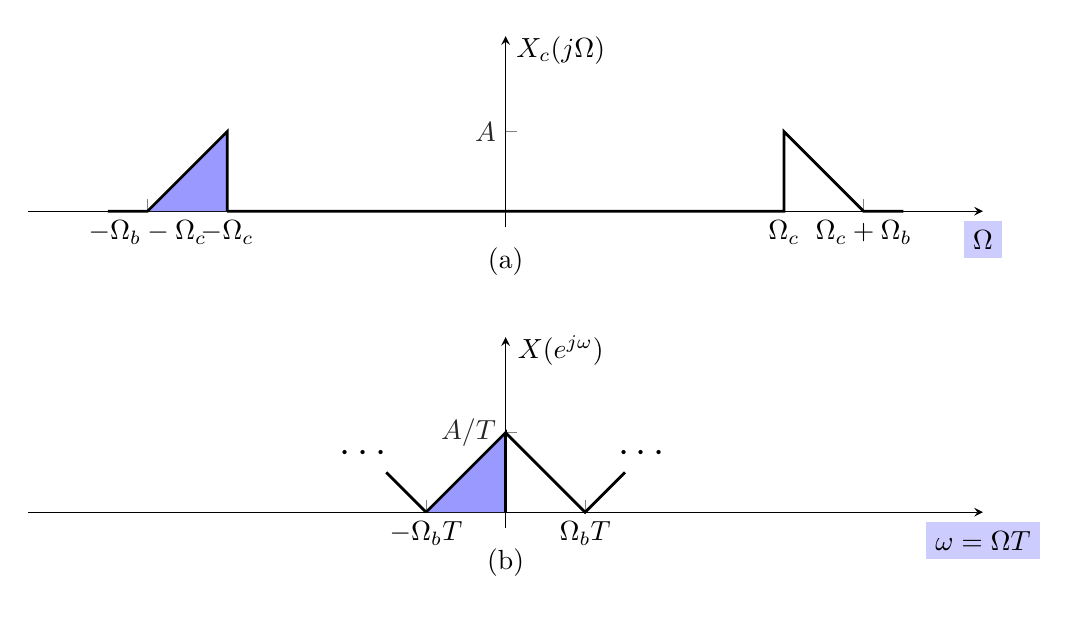
\begin{tikzpicture}
\begin{axis}[
	name=plot1,
	axis lines*=middle,
	enlargelimits = true,
	clip=true,
	scale only axis,
	width=\textwidth,
	height=0.2\textwidth,
	ymin=0, ymax=2,
	xmin=-10, xmax=10,
	axis line style={->,>=stealth},
	xlabel={ \tikz[baseline]{\node[fill=blue!20,anchor=base] (t1) {$\Omega$};}},
	ylabel={ $X_c(j\Omega)$},
	every axis x label/.style={
		at={(ticklabel* cs:1)},
		anchor=north,
	},
	every axis y label/.style={
		at={(ticklabel* cs:0.8)},
		anchor=south,
		xshift=0.7cm,
	},	
	ytick=1,
	yticklabels={ $A$},
	xtick={-9, -7, 0, 7, 9},
	xticklabels={ $-\Omega_b-\Omega_c$,  $-\Omega_c$,  0,  $\Omega_c$,  $\Omega_c+\Omega_b$}, 
	every outer y axis line/.append style={white!15!black},
	every y tick label/.append style={font=\color{white!15!black}},
	legend style={draw=white!15!black,fill=white,legend cell align=left}]
	\addplot[solid, line width=1pt] coordinates {(-7, 0) (7, 0) (7, 1) (9, 0) (10, 0)};
    \addplot[solid, fill=blue!40, line width=1pt] coordinates {(-10, 0) (-9, 0) (-7, 1) (-7, 0)};
\end{axis}

\begin{axis}[
	name=plot2,
    at=(plot1.below south east), anchor=above north east, yshift=-0.75cm,
	axis lines*=middle,
	enlargelimits = true,
	clip=true,
	scale only axis,
	width=\textwidth,
	height=0.2\textwidth,
	ymin=0, ymax=2,
	xmin=-10, xmax=10,
	axis line style={->,>=stealth},
	xlabel={ \tikz[baseline]{\node[fill=blue!20,anchor=base] (t1) {$\omega = \Omega T$};}},
	ylabel={ $X(e^{j\omega})$},
	every axis x label/.style={
		at={(ticklabel* cs:1)},
		anchor=north,
	},
	every axis y label/.style={
		at={(ticklabel* cs:0.8)},
		anchor=south,
		xshift=0.7cm,
	},	
	ytick=1,
	yticklabels={ $A/T$},
	xtick={-2, 2},
	xticklabels={ $-\Omega_bT$,  $\Omega_bT$}, 
	every outer y axis line/.append style={white!15!black},
	every y tick label/.append style={font=\color{white!15!black}},
	legend style={draw=white!15!black,fill=white,legend cell align=left}]
	\addplot[solid, line width=1pt] coordinates {(0, 1) (2, 0) (3, 0.5)};
    \addplot[solid, fill=blue!40, line width=1pt] coordinates {(-2, 0) (0, 1) (0, 0)};
    
    \addplot[solid, line width=1pt] coordinates {(-3, 0.5) (-2, 0)};
    \node[above] at (axis cs: -3.5, 0.5) {\Large $\cdots$};
    \node[above] at (axis cs: 3.5, 0.5) {\Large $\cdots$};
\end{axis}
\node[below, inner sep=0.25cm] at (plot1.south) {(a)};
\node[below, inner sep=0.25cm] at (plot2.south) {(b)};

\end{tikzpicture}
}
    \caption{Bandpass sampling.} \label{fig:bp_spectrum1}
\end{figure}


\begin{description}
\item[(a)] (2 points) What is the sampling frequency necessary to perform Nyquist sampling of the bandpass signal $x_c(t)$?
\if\SOLUTIONS1
{\color{\SolutionsColor}
\begin{align*}
\Omega_{s} = 2(\Omega_c + \Omega_b)
\end{align*}
}
\else\vspace{1cm}
\fi

\item[(b)] (6 points) Suppose that $\Omega_c = 8\pi$ rad/s and $\Omega_b = \pi$ rad/s. Draw the spectrum of $x[n]$ when $x_c(t)$ is sampled with sampling frequency $\Omega_s = 2\pi$ rad/s  (much smaller than the Nyquist rate). 

\begin{figure}[!h]
\centering
	\resizebox{\textwidth}{!}{\begin{tikzpicture}
\begin{axis}[
	name=plot1,
	axis lines*=middle,
	enlargelimits = false, clip=true,
	scale only axis,
	width=\textwidth,
	height=0.2\textwidth,
	ymin=0, ymax=1.5,
	xmin=-6, xmax=6,
	axis line style={->,>=stealth, shorten >= -0.7cm},
	xlabel={ \tikz[baseline]{\node[fill=blue!20,anchor=base] (t1) {$\omega$};}},
	ylabel={ $X(e^{j\omega})$},
	every axis x label/.style={
		at={(ticklabel* cs:1)},
		anchor=north,
        xshift=0.6cm,
	},
	every axis y label/.style={
		at={(ticklabel* cs:1)},
		anchor=south,
		xshift=0.7cm,
	},	
	ytick=1,
    yticklabels={$A/T$},
	xtick={-6,-4,...,6},
	xticklabels={$-3\pi$, $-2\pi$,  $-\pi$, $0$, $\pi$, $2\pi$, $3\pi$}, 
    xmajorgrids,
	every outer y axis line/.append style={white!15!black},
	every y tick label/.append style={font=\color{white!15!black}},
	legend style={draw=white!15!black,fill=white,legend cell align=left}]
    \if\SOLUTIONS1
      \ifdefined\SolD
        \def\fs{4}
        \foreach \k in {-1, 0, 1} {
          \addplot[solid, line width=1pt] coordinates {(0-\k*\fs-\fs/2, 0) (0-\k*\fs-\fs/2, 1) (2-\k*\fs-\fs/2, 0)};
          \addplot[solid, fill=blue!40, line width=1pt] coordinates {(-2-\k*\fs+\fs/2, 0) (0-\k*\fs+\fs/2, 1) (0-\k*\fs+\fs/2, 0)};
          }
      \else
      	\def\fs{4}
        \foreach \k in {-1, 0, 1} {
          \addplot[solid, line width=1pt] coordinates {(0-\k*\fs, 1) (2-\k*\fs, 0)};
          \addplot[solid, fill=blue!40, line width=1pt] coordinates {(-2-\k*\fs, 0) (0-\k*\fs, 1) (0-\k*\fs, 0)};
      }
      \fi
   \fi
\end{axis}
\end{tikzpicture}}\label{fig:bp_spectrum_sol1}
\end{figure}
\if\SOLUTIONS0\vspace{5cm}
\fi

\item[(c)] (7 points) In part (b) you saw that there is no spectrum overlap, even though $x_c(t)$ was sampled below the Nyquist rate. Is that always possible? Give conditions on the sampling frequency $\Omega_s$ in terms of $\Omega_c$ and $\Omega_b$ so that: (i) the spectrum is centered around $\omega = 0$ as in Figure~\ref{fig:bp_spectrum1}b, \underline{and} (ii) such that there is no spectrum overlap. 

\textit{Hint:} The spectrum replicas occur according to the sampling equation:
\begin{equation}
X(e^{j\Omega T}) = \frac{1}{T}\sum_{k=-\infty}^\infty X_c(j(\Omega-k\Omega_s))
\end{equation}

\if\SOLUTIONS1
{\color{\SolutionsColor}
Staring with the sampling equation we have the following conditions:

(i) In order to bring the signal down to baseband:
\begin{align*}
0 - k\Omega_s = \Omega_c \implies \Omega_c = -k\Omega_s
\end{align*}
for some negative integer $k$.

(ii) The ($-k-1$)th spectrum replica must fall at least at $-2\Omega_b$ in order to avoid spectrum overlap. Therefore, 
\begin{align*} \nonumber
-2\Omega_b - (k-1)\Omega_s &\geq \Omega_c \\ \nonumber
-2\Omega_b - (k-1)\Omega_s &\geq -k\Omega_s \tag{since $\Omega_c = -k\Omega_s$} \\
\Omega_s &\geq 2\Omega_b
\end{align*}
}
\else\vspace{10cm}
\fi


\item[(d)] (5 points) Repeat part (b), but now assume that $\Omega_c = 7\pi$ rad/s and $\Omega_b = \pi$ rad/s. Sampling is still performed with sampling frequency $\Omega_s = 2\pi$ rad/s. 

\textit{Note:} Although there isn't spectrum overlap in this case either, further processing would be necessary to center the spectrum around $\omega = 0$, as in Figure~\ref{fig:bp_spectrum1}b.

\begin{figure}[!h]
\centering
	\def\SolD{1}
	\resizebox{\textwidth}{!}{\begin{tikzpicture}
\begin{axis}[
	name=plot1,
	axis lines*=middle,
	enlargelimits = false, clip=true,
	scale only axis,
	width=\textwidth,
	height=0.2\textwidth,
	ymin=0, ymax=1.5,
	xmin=-6, xmax=6,
	axis line style={->,>=stealth, shorten >= -0.7cm},
	xlabel={ \tikz[baseline]{\node[fill=blue!20,anchor=base] (t1) {$\omega$};}},
	ylabel={ $X(e^{j\omega})$},
	every axis x label/.style={
		at={(ticklabel* cs:1)},
		anchor=north,
        xshift=0.6cm,
	},
	every axis y label/.style={
		at={(ticklabel* cs:1)},
		anchor=south,
		xshift=0.7cm,
	},	
	ytick=1,
    yticklabels={$A/T$},
	xtick={-6,-4,...,6},
	xticklabels={$-3\pi$, $-2\pi$,  $-\pi$, $0$, $\pi$, $2\pi$, $3\pi$}, 
    xmajorgrids,
	every outer y axis line/.append style={white!15!black},
	every y tick label/.append style={font=\color{white!15!black}},
	legend style={draw=white!15!black,fill=white,legend cell align=left}]
    \if\SOLUTIONS1
      \ifdefined\SolD
        \def\fs{4}
        \foreach \k in {-1, 0, 1} {
          \addplot[solid, line width=1pt] coordinates {(0-\k*\fs-\fs/2, 0) (0-\k*\fs-\fs/2, 1) (2-\k*\fs-\fs/2, 0)};
          \addplot[solid, fill=blue!40, line width=1pt] coordinates {(-2-\k*\fs+\fs/2, 0) (0-\k*\fs+\fs/2, 1) (0-\k*\fs+\fs/2, 0)};
          }
      \else
      	\def\fs{4}
        \foreach \k in {-1, 0, 1} {
          \addplot[solid, line width=1pt] coordinates {(0-\k*\fs, 1) (2-\k*\fs, 0)};
          \addplot[solid, fill=blue!40, line width=1pt] coordinates {(-2-\k*\fs, 0) (0-\k*\fs, 1) (0-\k*\fs, 0)};
      }
      \fi
   \fi
\end{axis}
\end{tikzpicture}} \label{fig:bp_spectrum_sol1}
\end{figure}
\if\SOLUTIONS0\vspace{5cm}
\fi

\end{description}

\newpage
\section*{Problem 4: (20 points)}
The diagram of Figure~\ref{fig:sampling_diagram} represents the initial DSP of a high-speed application. Since fast ADCs are expensive, the design engineers decided to perform Nyquist-rate sampling and upsample the signal immediately after the ADC, as illustrated in Figure~\ref{fig:sampling_diagram}. The lowpass filter $H(z)$ after upsampling is used to eliminate unwanted spectrum replicas of the signal and of quantization noise. The additive white  noise introduced by the quantizer has average power $\sigma_Q^2$.

\begin{figure}[!h]
\centering
	\resizebox{\textwidth}{!}{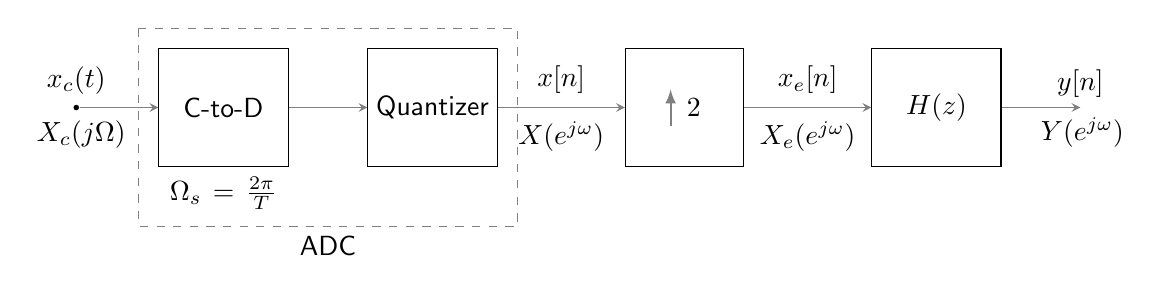
\begin{tikzpicture}[->, >=stealth, shorten >= 0pt, draw=black!50, node distance=3.2cm, font=\sffamily]
    \tikzstyle{node}=[circle,fill=black,minimum size=2pt,inner sep=0pt]
    \tikzstyle{block}=[draw=black,rectangle,fill=none,minimum size=1.5cm, inner sep=2pt]

	\node[node] (xc) {};    
    \node[block, right=1cm of xc, text width = 1.5cm, align= center] (CTD) {C-to-D};
    \node[block, right=1cm of CTD, text width = 1.5cm, align= center] (Q) {Quantizer};
    \node[block, right of=Q, text width = 1cm, align= center] (L) {$~~2$};
    \draw[-latex, shorten >= 15pt, shorten <= 15pt, line width=0.75pt] ($(L.south)-(5pt, 0)$) -- ($(L.north)-(5pt, 0)$) {};
    \node[block, right of=L, text width = 1.5cm, align= center] (H) {$H(z)$};
    \coordinate[right=1cm of H] (yc) {};
    
    \path (xc) edge (CTD);
    \path (CTD) edge (Q);
    \path (Q) edge (L);
    \path (L) edge (H);
    \path (H) edge (yc);
    
    \coordinate (mid1) at ($(Q.east)!0.5!(L.west)$);
    \coordinate (mid2) at ($(L.east)!0.5!(H.west)$);
    
    \node[above = 0.5mm of mid1] {$x[n]$};
    \node[below = 0.5mm of mid1] {$X(e^{j\omega})$};
    \node[above = 0.5mm of mid2] {$x_e[n]$};
    \node[below = 0.5mm of mid2] {$X_e(e^{j\omega})$};
    \node[above = 0mm of xc, text width = 1cm, align=center] {$x_c(t)$};
    \node[below = 0mm of xc, text width = 1cm, align=center] {$X_c(j\Omega)$};
    \node[above = 0mm of yc, text width = 1cm, align=center] {$y[n]$};
    \node[below = 0mm of yc, text width = 1cm, align=center] {$Y(e^{j\omega})$};
    \node[align=center, text width=2cm, below] at ($(CTD.south)$) {$\Omega_s = \frac{2\pi}{T}$};
    
    \draw[dashed] ($(CTD.north west)+(-0.25cm, 0.25cm)$) rectangle ($(Q.south east)+(0.25, -0.75cm)$);
    \node[below] at ($(CTD.south west)!0.5!(Q.south east) -(0, 0.75cm)$) {ADC};
\end{tikzpicture}} 
    \caption{Block diagram of system for problem 4.}\label{fig:sampling_diagram}
\end{figure}

\begin{description}
\item[(a)] (8 points) The plot below shows the spectrum $X(e^{j\omega})$ with signal (triangular shape) and quantization noise (dashed red line) components. Use the empty graphs below to sketch $X_e(e^{j\omega})$ and $Y(e^{j\omega})$. In your plots, draw both the signal and noise components. Assume that $H(z)$ is the ideal lowpass filter with cutoff frequency $\pm\pi/2$ and \underline{unit gain}.

\textit{Hint:} consider signal and noise separately.
 
\FloatBarrier
\begin{figure}[!h]
\centering
	\resizebox{0.9\textwidth}{!}{% \fs and \fmax must be defined before calling this picture.
\def\fs{5}
\def\fmax{2.5}
\begin{tikzpicture}
\begin{axis}[
	name=plot2,
	%at=(plot1.below south east), anchor=above north east,
	axis lines*=middle,
	enlargelimits = true,
	clip=true,
	scale only axis,
	width=\textwidth,
	height=0.2\textwidth,
	ymin=0,
	ymax=3,
	xmin=-\fs-1,
	xmax=\fs+1,
	axis line style={->,>=stealth},
	xlabel={\small \tikz[baseline]{\node[fill=blue!20,anchor=base] (t1) {$\omega = \Omega T$};}},
	ylabel={\small $X(e^{j\omega})$},
	every axis x label/.style={
		at={(ticklabel* cs:1)},
		anchor=north,
	},
	every axis y label/.style={
		at={(ticklabel* cs:0.8)},
		anchor=south,
		xshift=0.6cm,
	},
	xtick=\empty,
	ytick=2,
	yticklabels={\small $\frac{1}{T}$},
	yticklabel style={yshift=0.1cm},
	xtick={-\fs, -2.5, 0, 2.5, \fs},
	xticklabels={\small $-2\pi$, \small $-\pi$, \small 0, \small $\pi$, \small $2\pi$}, 
	every outer y axis line/.append style={white!15!black},
	every y tick label/.append style={font=\color{white!15!black}},
	legend style={draw=white!15!black,fill=white,legend cell align=left}]
	\addplot[solid, line width=1pt] coordinates {(0, 2) (2.5, 0) (0, 0)};
	\addplot[solid, line width=1pt, fill=blue!50] coordinates {(0, 2) (-2.5, 0) (0, 0)};
	\addplot[solid, line width=1pt] coordinates {(\fs, 2) (\fs+2.5, 0) (\fs, 0)};
	\addplot[solid, line width=1pt, fill=blue!50] coordinates {(\fs, 2) (\fs-2.5, 0) (\fs, 0)};
	\addplot[solid, line width=1pt] coordinates {(-\fs, 2) (-\fs+2.5, 0) (-\fs, 0)};
	\addplot[solid, line width=1pt, fill=blue!50] coordinates {(-\fs, 2) (-\fs-2.5, 0) (-\fs, 0)};
	\addplot[solid, line width=1pt] coordinates {(-2*\fs, 2) (-2*\fs+2.5, 0) (-2*\fs, 0)};
	\addplot[solid, line width=1pt, fill=blue!50] coordinates {(-2*\fs, 2) (-2*\fs-2.5, 0) (-2*\fs, 0)};]
	\addplot[solid, line width=1pt] coordinates {(2*\fs, 2) (2*\fs+2.5, 0) (2*\fs, 0)};
	\addplot[solid, line width=1pt, fill=blue!50] coordinates {(2*\fs, 2) (2*\fs-2.5, 0) (2*\fs, 0)};
    \addplot[red2, line width=1.5pt, dashed] coordinates {(-3*\fs, 0) (-3*\fs, 0.7) (3*\fs, 0.7) (3*\fs, 0)} node[pos=0.57, black, pin={[pin edge={red, solid, thick}]30:{$\sigma_Q^2$}}, inner sep=0pt] {};
\end{axis}

\def\fsM{2.5}
\def\fmaxM{1.25} % 
\def\BWM{1.25} % WN * T_d = WN * 2 * T = 2 * (BW)
\begin{axis}[
	name=plot3,
	at=(plot2.below south east), anchor=above north east,
	axis lines*=middle,
	enlargelimits = true,
	clip=true,
	scale only axis,
	width=\textwidth,
	height=0.2\textwidth,
	ymin=0,
	ymax=3,
	xmin=-\fs-1,
	xmax=\fs+1,
	axis line style={->,>=stealth},
	xlabel={\small \tikz[baseline]{\node[fill=blue!20,anchor=base] (t1) {$\omega = \frac{\Omega T}{2}$};}},
	ylabel={\small $X_e(e^{j\omega}) = X(e^{j\omega L})$},
	every axis x label/.style={
		at={(ticklabel* cs:1)},
		%xshift=0.2cm,
		anchor=north,
	},
	every axis y label/.style={
		at={(ticklabel* cs:0.8)},
		anchor=south,
		xshift=1.5cm,
	},
	xtick=\empty,
	ytick=2,
	yticklabels={\small $\frac{1}{T}$},
	xtick={-5, -3.75, ..., 5},
	xticklabels={\small $-2\pi$, \small $-\frac{3\pi}{2}$, \small $-\pi$, \small $-\frac{\pi}{2}$, 0, \small $\frac{\pi}{2}$, \small $\pi$, \small $\frac{3\pi}{2}$, \small $2\pi$}, 
	every outer y axis line/.append style={white!15!black},
	every y tick label/.append style={font=\color{white!15!black}},
	legend style={draw=white!15!black,fill=white,legend cell align=left}]
    \if\SOLUTIONS1
	\addplot[solid, line width=1pt] coordinates {(0, 2) (\BWM, 0) (0, 0)};
	\addplot[solid, line width=1pt, fill=blue!50] coordinates {(0, 2) (-\BWM, 0) (0, 0)};
	\addplot[solid, line width=1pt] coordinates {(\fsM, 2) (\fsM+\BWM, 0) (\fsM, 0)};
	\addplot[solid, line width=1pt, fill=blue!50] coordinates {(\fsM, 2) (\fsM-\BWM, 0) (\fsM, 0)};
	\addplot[solid, line width=1pt] coordinates {(-\fsM, 2) (-\fsM+\BWM, 0) (-\fsM, 0)};
	\addplot[solid, line width=1pt, fill=blue!50] coordinates {(-\fsM, 2) (-\fsM-\BWM, 0) (-\fsM, 0)};
	\addplot[solid, line width=1pt] coordinates {(-2*\fsM, 2) (-2*\fsM+\BWM, 0) (-2*\fsM, 0)};
	\addplot[solid, line width=1pt, fill=blue!50] coordinates {(-2*\fsM, 2) (-2*\fsM-\BWM, 0) (-2*\fsM, 0)};]
	\addplot[solid, line width=1pt] coordinates {(2*\fsM, 2) (2*\fsM+\BWM, 0) (2*\fsM, 0)};
	\addplot[solid, line width=1pt, fill=blue!50] coordinates {(2*\fsM, 2) (2*\fsM-\BWM, 0) (2*\fsM, 0)};
	\node[scale=1, fill=black!20] at (axis cs: 5, 2) {Upsampled by 2};
    \addplot[red2, line width=1.5pt, dashed] coordinates {(-3*\fs, 0) (-3*\fs, 0.7) (3*\fs, 0.7) (3*\fs, 0)} node[pos=0.45, black, pin={[pin edge={red, solid, thick}]30:{$\sigma_Q^2$}}, inner sep=0pt] {};
    \fi
\end{axis}

\def\fbw{1.25}
\begin{axis}[
	name=plot4,
	at=(plot3.below south east), anchor=above north east,
	axis lines*=middle,
	enlargelimits = true, clip=true,
	scale only axis,
	width=\textwidth,
	height=0.2\textwidth,
	ymin=0,
	ymax=3,
	xmin=-\fs-1,
	xmax=\fs+1,
	axis line style={->,>=stealth},
	xlabel={\small \tikz[baseline]{\node[fill=blue!20,anchor=base] (t1) {$\omega = \frac{\Omega T}{2}$};}},
	ylabel={\small $Y(e^{j\omega})$},
	every axis x label/.style={
		at={(ticklabel* cs:1)},
		%xshift=0.2cm,
		anchor=north,
	},
	every axis y label/.style={
		at={(ticklabel* cs:0.8)},
		anchor=south,
		xshift=0.6cm,
	},
	xtick=\empty,
    ytick=2,
    yticklabels={\small $\frac{1}{T}$},
	yticklabel style={yshift=0.2cm},
	xtick={-5, -3.75, ..., 5},
	xticklabels={\small $-2\pi$, \small $-\frac{3\pi}{2}$, \small $-\pi$, \small $-\frac{\pi}{2}$, 0, \small $\frac{\pi}{2}$, \small $\pi$, \small $\frac{3\pi}{2}$, \small $2\pi$}, 
	every outer y axis line/.append style={white!15!black},
	every y tick label/.append style={font=\color{white!15!black}},
	legend style={draw=white!15!black,fill=white,legend cell align=left}]
    \if\SOLUTIONS1
	\addplot[solid, line width=1pt] coordinates {(0, 2) (\BWM, 0) (0, 0)};
	\addplot[solid, line width=1pt, fill=blue!50] coordinates {(0, 2) (-\BWM, 0) (0, 0)};
	\addplot[solid, line width=1pt] coordinates {(-2*\fsM, 2) (-2*\fsM+\BWM, 0) (-2*\fsM, 0)};
	\addplot[solid, line width=1pt, fill=blue!50] coordinates {(-2*\fsM, 2) (-2*\fsM-\BWM, 0) (-2*\fsM, 0)};]
	\addplot[solid, line width=1pt] coordinates {(2*\fsM, 2) (2*\fsM+\BWM, 0) (2*\fsM, 0)};
	\addplot[solid, line width=1pt, fill=blue!50] coordinates {(2*\fsM, 2) (2*\fsM-\BWM, 0) (2*\fsM, 0)};
    \addplot[red2, line width=1.5pt, dashed] coordinates {(-2*\fsM-\BWM, 0) (-2*\fsM-\BWM, 0.75) (-2*\fsM+\BWM, 0.75) (-2*\fsM+\BWM, 0) (-\BWM, 0) (-\BWM, 0.75) (\BWM, 0.75) (\BWM, 0) (2*\fsM-\BWM, 0) (2*\fsM-\BWM, 0.75) (2*\fsM-\BWM, 0.75) (2*\fsM+\BWM, 0.75) (2*\fsM+\BWM, 0)} node[pos=0.57, black, pin={[pin edge={red, solid, thick}]30:{$\sigma_Q^2$}}, inner sep=0pt] {};
    \fi
\end{axis}

\end{tikzpicture}
} \label{fig:spectrum_upsample}
\end{figure}
\FloatBarrier

\item[(b)] (6 points) Now assume that $H(z)$ is the first-order lowpass filter given by
\begin{equation}
H(z) = \frac{1 + cz^{-1}}{1 - cz^{-1}}, \qquad 0 < c < 1.
\end{equation}

Assume that this filter is implemented using the transposed direct form II with signal values and filter coefficients scaled as Q15 integers. The result of multiplications is quantized to 16-bits (15 bits plus sign) \underline{immediately after} the multiplications and \underline{before} any additions are done. Draw the signal flow graph diagram of this system. In your drawing include noise sources representing the quantization of the multiplications. Label each noise source with average power $\sigma_{15}^2$. You may combine noise sources whenever possible. In addition, circle \underline{all nodes} in which overflow may happen.

\textit{Note:} You do not need to include noise sources in multiplications by 1.

\if\SOLUTIONS1
{\color{\SolutionsColor}
Overflow may happen in any node in which additions are performed. Multiplications do not overflow. 

The noise sources were combined into one with average power $2\sigma_{15}^2$. Note that since $b_0 = 1$, in this case, then this multiplication is not performed and therefore we should not include a noise source for it.

\FloatBarrier
\begin{figure}[h!]
\centering
	\def\SolD{1}
	\resizebox{0.5\textwidth}{!}{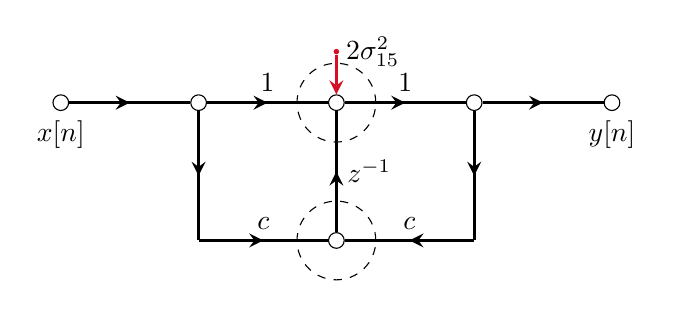
\begin{tikzpicture}[node distance=1.75cm]
\tikzstyle{node}=[circle,fill=red2,minimum size=2pt,inner sep=0pt]
%Place the nodes
\node[terminal={below}{$x[n]$}] (x) at (0,0) {};
\node[terminal={below}{}, right of=x] (00) {};
\node[terminal={below}{}, right of= 00] (01) {};
\node[terminal={below}{}, right of=01] (02) {};
\node[terminal={below}{$y[n]$}, right of=02] (y) {};

\foreach \j in {1} {
	\pgfmathtruncatemacro{\jn}{(\j-1)}%
	\coordinate[below of=\jn0] (\j0) {};
	\node[terminal={below}{}, below of=\jn1] (\j1) {};
	\coordinate[below of=\jn2] (\j2) {};
}

%
\draw[zpath={right}] (11) to (01);

%
\draw[amark] (00) to (10);
\draw[amark] (02) to (12);


%
\draw[amark={$1$}{above}] (00) to (01);
\draw[amark={$c$}{above}] (10) to (11);

%
\draw[amark={$1$}{above}] (01) to (02);
\draw[amark={$c$}{above}] (12) to (11);


\draw[amark] (x) to (00);
\draw[amark] (02) to (y);

\draw[dashed] (01) circle[radius=0.5cm];
\draw[dashed] (11) circle[radius=0.5cm];

\node[node, above=0.5cm of 01] (E) {}; \node[right] at (E) {$2\sigma_{15}^2$};
\draw[->, >=stealth, red2, \thickness] (E) to (01);

\end{tikzpicture}}
\end{figure}
\FloatBarrier
}
\else\vspace{7cm}
\fi

\item{(c)} (6 points) Write an equation for the PSD of the total noise at the output of $H(z)$. The total noise includes quantization noise from the quantizer and roundoff noise from your filter implementation in part (b). Write your answer in terms of $\sigma_{15}^2$, $\sigma_{Q}^2$, and $c$.

\if\SOLUTIONS1
{\color{\SolutionsColor}
Using superposition, we see that the quantization noise is filtered by $H(z)$, while the roundoff noise is filtered only by the poles of $H(z)$, which we'll denoted by $\frac{1}{A(z)}$. Therefore,

\begin{align*}
\Phi_{ff}(e^{j\omega}) &= \sigma_Q^2|H(e^{j\omega})|^2 + 2\sigma_{15}^2\frac{1}{|A(e^{j\omega})|} \\
&= \sigma_Q^2|H(e^{j\omega})|^2 + 2\sigma_{15}^2\frac{1}{|A(e^{j\omega})|} \\
& = \frac{\sigma_Q^2(1 + c^2 + 2c\cos\omega) + 2\sigma_{15}^2}{1 + c^2 - 2c\cos\omega}
\end{align*}

}
\else\vspace{5cm}
\fi
\end{description}


\end{document}
